\documentclass[11pt,a4paper]{article}
\usepackage[utf8]{inputenc}
\usepackage[T1]{fontenc}
\usepackage[ngerman]{babel}
\usepackage{lmodern}
\usepackage{microtype}
\usepackage{booktabs}
\usepackage{longtable}
\usepackage[hidelinks]{hyperref}
\usepackage{graphicx}
\usepackage{forest}
\usepackage[backend=bibtex,style=numeric,sorting=none]{biblatex}
\addbibresource{refs.bib}
\title{Wie wirken soziale Medien auf Aufmerksamkeit?}
\author{ScienceKG -- Automatisch generierte Tiefenanalyse}
\date{\today}
\begin{document}
\begin{titlepage}
\centering
{\large ScienceKG \textendash{} Tiefenanalyse\par}
\vspace{2.5cm}
{\huge\bfseries Wie wirken soziale Medien auf Aufmerksamkeit?\par}
\vspace{2cm}
{\large Automatisch generierte wissenschaftliche Ausarbeitung\par}
\vfill
{\large \today\par}
\end{titlepage}
\tableofcontents
\newpage
\section{Einleitung}

Text mit Beleg \autocite{arxiv_2310_12345}.

\section{Kapitel Eins}

\subsection{Unterfrage 1a}

Befund \autocite{arxiv_2310_12345}.

\section{Fazit}

Schluss.
\appendix
\section{Anhang: Forschungsstruktur, Diagramme und Tabellen}
\begin{figure}[h]
\centering
\begin{forest}
for tree={draw, rounded corners, font=\footnotesize, grow=east, edge={->, >=latex}, anchor=west, align=left, text width=3.2cm, l sep=12mm, s sep=2mm}
[{Wie wirken soziale Medien?}[{Kapitel Eins}[{Unterfrage 1a}]]]
\end{forest}
\caption{Struktur der Tiefenanalyse: Forschungsfrage und untersuchte Teilfragen.}
\end{figure}
\begin{figure}[h]
\centering
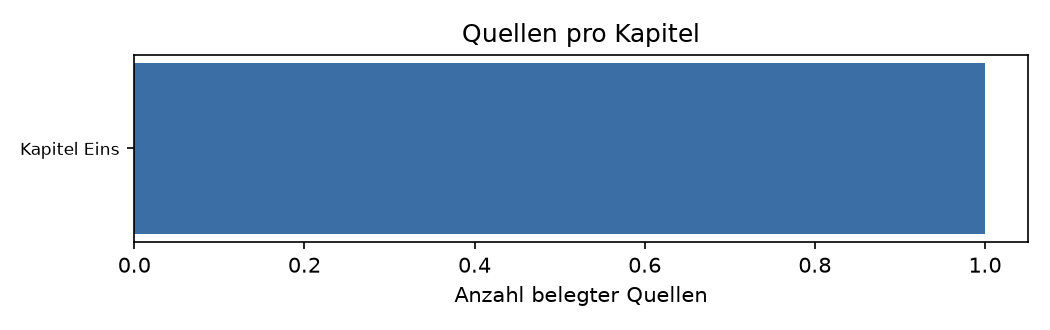
\includegraphics[width=0.85\textwidth]{chart_sources.png}
\caption{Anzahl der belegten Quellen je Kapitel.}
\end{figure}

\begin{figure}[h]
\centering
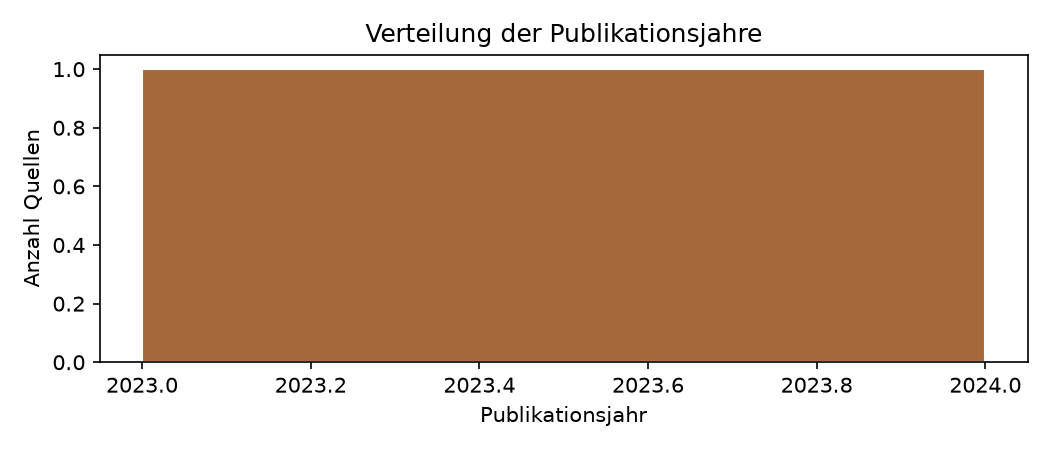
\includegraphics[width=0.85\textwidth]{chart_years.png}
\caption{Verteilung der Publikationsjahre der zitierten Quellen.}
\end{figure}
\begin{longtable}{p{0.62\textwidth} r r}
\caption{Überblick der untersuchten Kapitel.}\\
\toprule
\textbf{Kapitel} & \textbf{Teilfragen} & \textbf{Quellen} \\
\midrule
\endhead
Kapitel Eins & 1 & 1 \\
\bottomrule
\end{longtable}
\begin{longtable}{r p{0.5\textwidth} c p{0.22\textwidth}}
\caption{Übersicht der einbezogenen Quellen.}\\
\toprule
\# & \textbf{Titel} & \textbf{Jahr} & \textbf{ID} \\
\midrule
\endhead
1 & Attention Paper & 2023 & arxiv:2310.12345 \\
\bottomrule
\end{longtable}
\printbibliography[title={Quellenverzeichnis}]
\end{document}
